\section{排序关系}
不同于等价关系,\DefineConcept{排序关系}(ordering relation)具有一些别致的性质.

\subsection{偏序关系}
\begin{definition}
%@see: 《Elements of Set Theory》 P168. Definition
设\(\rel{R}\)是集合\(A\)上的一个二元关系.
如果\(\rel{R}\)具有\emph{自反性}、\emph{反对称性}和\emph{传递性},
那么称“\(\rel{R}\)是\(A\)上的\DefineConcept{偏序关系}(partial ordering)”,
称“\(A\)是\DefineConcept{偏序集}(partially ordered set)”.
\end{definition}

\begin{example}
%@see: 《Real Analysis Modern Techniques and Their Applications Second Edition》 P5.
设\(A\)是集合,
则\(\subseteq\)是\(\Powerset A\)上的偏序关系.
\end{example}

\subsection{最大元,最小元,上界,下界}
\begin{definition}
设\(X\)是非空集合,
\(x \in X\),
\(E \subseteq X\),
\(\rel{R}\)是\(X\)上的偏序关系.

我们如果把满足\[
	[y \in X \implies x\rel{R}y]
	\implies
	y = x,
\]的\(x\)称作“\(X\)的\DefineConcept{最大元}(maximal element)”,
那么相应地把满足\[
	[y \in X \implies y\rel{R}x]
	\implies
	y = x,
\]的\(x\)称作“\(X\)的\DefineConcept{最小元}(minimal element)”.
在这样的语境下,
如果\(x\)满足\[
	(\forall y \in E)[y\rel{R}x],
\]
那么称“\(x\)是\(E\)的\DefineConcept{上界}(upper bound)”.
如果\(x\)满足\[
	(\forall y \in E)[x\rel{R}y],
\]
那么称“\(x\)是\(E\)的\DefineConcept{下界}(lower bound)”.
\end{definition}

\subsection{线性序}
\begin{definition}
%@see: 《Elements of Set Theory》 P62. Definition
设\(\rel{R}\)是集合\(A\)上的一个二元关系.
如果\begin{enumerate}
	\item \(\rel{R}\)具有传递性,
	\item \(\rel{R}\)在\(A\)上服从\DefineConcept{三一律}(trichotomy),
	也就是说,对于\(\forall x,y \in A\),
	在以下三个命题中,有且仅有一个是真命题:\[
		x \rel{R} y, \qquad
		x = y, \qquad
		y \rel{R} x;
	\]
	%@see: https://mathworld.wolfram.com/TrichotomyLaw.html
\end{enumerate}
那么称\(\rel{R}\)为
“\(A\)上的\DefineConcept{线性序}(linear ordering)
或\DefineConcept{全序}(total ordering)”.
\end{definition}

应该注意到,当\(x = y\)时,三一律要求\[
	x \rel{R} x, \qquad
	x = x, \qquad
	x \rel{R} x
\]中的一个成立,
考虑到\(x = x\)恒成立,
那么必有\(x \rel{R} x\)恒不成立.
易见当\(x \neq y\)时,必有\(x \rel{R} y\)或\(y \rel{R} x\)之一成立,
都不可能有\(x \rel{R} y\)和\(y \rel{R} x\)都成立.
于是我们证得如下定理.

\begin{theorem}
%@see: 《Elements of Set Theory》 P63. Theorem 3R
设\(\rel{R}\)是集合\(A\)上的线性序.
\begin{enumerate}
	\item \(\rel{R}\)不具有自反性,
	即不存在\(x\)使得\(x \rel{R} x\).

	\item \(\rel{R}\)在\(A\)上是连通的(\(\rel{R}\) is \emph{connected} on \(A\)),
	即对于不同的\(x,y \in A\),要么有\(x \rel{R} y\)成立,要么有\(y \rel{R} x\)成立.
\end{enumerate}
\end{theorem}

值得注意的是,
线性序\(\rel{R}\)永远不会给出如下的环形:
\begin{center}
	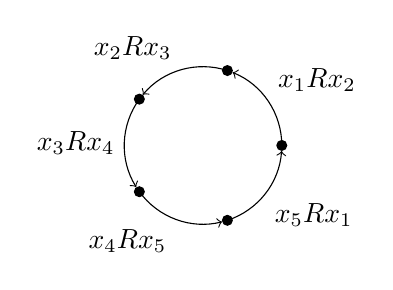
\begin{tikzpicture}
		\fill(1,0)circle(2pt)coordinate(A0);
		\fill({cos(72)},{sin(72)})circle(2pt)coordinate(A1);
		\fill({cos(144)},{sin(144)})circle(2pt)coordinate(A2);
		\fill({cos(216)},{sin(216)})circle(2pt)coordinate(A3);
		\fill({cos(288)},{sin(288)})circle(2pt)coordinate(A4);
		\begin{scope}[->]
			\draw(A0)arc[start angle=0,end angle=68,radius=1]node[midway,above right]{\(x_1 \rel{R} x_2\)};
			\draw(A1)arc[start angle=72,end angle=140,radius=1]node[midway,above left]{\(x_2 \rel{R} x_3\)};
			\draw(A2)arc[start angle=144,end angle=212,radius=1]node[midway,left]{\(x_3 \rel{R} x_4\)};
			\draw(A3)arc[start angle=216,end angle=284,radius=1]node[midway,below left]{\(x_4 \rel{R} x_5\)};
			\draw(A4)arc[start angle=288,end angle=356,radius=1]node[midway,below right]{\(x_5 \rel{R} x_1\)};
		\end{scope}
	\end{tikzpicture}
\end{center}
这是因为,如果我们有这样的环形成立,
那么根据传递性必有\(x_1 \rel{R} x_1\),
而这就与反自反性矛盾!

\begin{example}
设\(\rel{R}\)是\(A\)上的一个线性序,
证明:\(\rel{R}^{-1}\)也是\(A\)上的线性序.
\begin{proof}
由于\[
	\bigl( x \rel{R} y \land y \rel{R} z \implies x \rel{R} z \bigr)
	\iff
	\bigl( y \rel{R}^{-1} x \land z \rel{R}^{-1} y \implies z \rel{R}^{-1} x \bigr),
\]
可知\(\rel{R}^{-1}\)具有传递性.
又因为\(\rel{R}\)是\(A\)上的线性序,
所以对于\(\forall x,y \in A\),以下三个命题\[
	x \rel{R} y, \qquad
	x = y, \qquad
	y \rel{R} x
\]有且仅有一个成立;
换句话说,以下三个命题\[
	y \rel{R}^{-1} x, \qquad
	x = y, \qquad
	x \rel{R}^{-1} y
\]有且仅有一个成立;
可知\(\rel{R}^{-1}\)服从三一律.
综上所述,\(\rel{R}^{-1}\)也是\(A\)上的线性序.
\end{proof}
\end{example}
